\documentclass[article]{jss}

%%%%%%%%%%%%%%%%%%%%%%%%%%%%%%
%% declarations for jss.cls %%%%%%%%%%%%%%%%%%%%%%%%%%%%%%%%%%%%%%%%%%
%%%%%%%%%%%%%%%%%%%%%%%%%%%%%%

%% almost as usual
\author{Matthew K. Lau\\ Harvard Forest\\Harvard University \And
        Stuart R. Borrett\\Department of Biology and Marine Biology\\
        University of North Carolina Wilmington\\and\\Duke Network
        Analysis Center, Social Science Research Institute \\ Duke University}
\title{enaR: Ecosystem Network Analysis with R}

%% for pretty printing and a nice hypersummary also set:
\Plainauthor{Matthew K. Lau, Stuart R. Borrett} %% comma-separated
\Plaintitle{enaR: Ecosystem Network Analyses with R} %% without formatting
\Shorttitle{\pkg{enaR}: Ecosystem Network Analyses with R} %% a short title (if necessary)

%% an abstract and keywords
\Abstract{
  Ecosystem Network Analysis (ENA) provides a framework for
  investigating the structure, function and dynamics of ecological
  systems, primarily ecosystem models with physically conserved
  units. Here, we present the \textit{enaR} package, which provides a
  broad representation of many of the core tools developed by the ENA
  community, detailing how to use the primary functions of the package
  for the analysis of single models or simultaneous, synthetic
  analysis of multiple ecosystem models.
}
\Keywords{ecology, ENA, ecosystems, species interactions, networks, \proglang{R}}
\Plainkeywords{ecology, ENA, ecosystems, species interactions, networks, R} %% without formatting
%% at least one keyword must be supplied

%% publication information
%% NOTE: Typically, this can be left commented and will be filled out by the technical editor
%% \Volume{50}
%% \Issue{9}
%% \Month{June}
%% \Year{2012}
%% \Submitdate{2012-06-04}
%% \Acceptdate{2012-06-04}

%% The address of (at least) one author should be given
%% in the following format:

\Address{
  Matthew K. Lau\\
  Harvard Forest\\
  Harvard University\\
  324 N Main St, Petersham, MA 01366, USA\\
  E-mail: \email{matthewklau@fas.harvard.edu}\\
  URL: \url{https://github.com/MKLau}\\
  \\
  Stuart R. Borrett\\
  Department of Biology and Marine Biology\\
  University of North Carolina Wilmington\\
  601 South College Road, Wilmington, NC 28403, USA\\
  E-mail: \email{borretts@uncw.edu}\\
  URL: \url{http://people.uncw.edu/borretts/}
}

%% It is also possible to add a telephone and fax number
%% before the e-mail in the following format:
%% Telephone: +43/512/507-7103
%% Fax: +43/512/507-2851

%% for those who use Sweave please include the following line (with % symbols):
%% need no \usepackage{Sweave.sty}

\usepackage[super, sort]{natbib}
  \bibpunct{(}{)}{;}{a}{,}{,} % required for natbib
\usepackage{ucs} %needed for R output: signif stars etc, quotes
\usepackage[utf8x]{inputenc}
\usepackage[T1]{fontenc}
\usepackage{sidecap}

%% end of declarations %%%%%%%%%%%%%%%%%%%%%%%%%%%%%%%%%%%%%%%%%%%%%%%


\begin{document}

%% include your article here, just as usual
%% Note that you should use the \pkg{}, \proglang{} and \code{} commands.

\section[Ecosystem Network Analysis]{Ecosystem Network Analysis}
%% Note: If there is markup in \(sub)section, then it has to be escape as above.

Ecosystem Network Analysis (ENA) is a family of algorithms for
investigating the structure and function of ecosystems
\cite{borrett12_netecol}.  These systems are modeled as networks of
thermodynamically conserved energy--matter exchanges in which nodes
represent the species, groups of species, or non-living componets
(e.g., dead organic matter) of the ecosystem, and the weighted,
directed edges are the quantified transfers of energy or matter.  

Here we present an \R package that brings together multiple ENA
algorithms from several approaches into one common software framework
that is readily available and extensible.  The package builds on the
\textit{network} data structure developed by
\citet{butts08_network}. In addition to being able to perform several
types of ENA with a single package, users can also make use of network
analysis tools built into the \textit{network}, the \textit{sna}
(social network analysis) \citep{butts08_social}, and other components
of what is collectively called \textit{statnet}
\citep{handcock2008statnet}.


% objectives
Disparate software packages have been created to support
ENA. Initially algorithms were developed and distributed as the DOS
based NETWRK4, which is still available from \cite{ulanowiczCITE}.
Some of these algorithms were reimplemented in an Microsoft Excel
based toolbox, WAND \citep{allesina04_wand}. The popular Ecopath with
Ecosim software that assists with model construction
\citep{christensen04} also provides multiple ENA algorithms.  More
recently, \citet{fath06} published NEA.m that collects many ENA
algorithms together in a single MATLAB\copyright function. Although
these packages collectively provide access to a large set of powerful
analytical tools, the fragmented distribution of these algorithms has
inhibited the development of theory and the further implementation of
important aoglorithms. One objective for this \R\ package is to bring
together these different algorithms into a single package that is both
accessible and extensible.






%% <<z,echo=false>>=
%% # set plotting parameters
%% opar <- par(las=1,mar=c(0,0,0,0),xpd=TRUE,bg="white")

%% ## Taken from https://stat.ethz.ch/pipermail/r-devel/2011-September/062126.html
%% if (all(ls()!='f.list')){
%%   require(codetools)
%% library(enaR)
%% called.by <- function(tarFunc, tarPack){
%%   flist <-   sapply(lsf.str(tarPack, all=TRUE), c)
%%   names(flist) <- NULL
%%   gotit <- sapply(flist, function(x) tarFunc %in% findGlobals(get(x, tarPack),FALSE)$functions)
%%   flist[gotit]
%% }

%% f.list <- as.character(sapply(lsf.str('package:enaR',all=TRUE),c))
%% f.array <- array(0,dim=rep(length(f.list),2))
%% rownames(f.array) <- colnames(f.array) <- f.list
%% for (i in 1:length(f.list)){
%%   f.array[match(called.by(f.list[i],'package:enaR'),rownames(f.array)),i] <- 1
%% }
%% f.net <- network(t(f.array))
%% }

%% plot(f.net,displaylabels=TRUE,label.cex=0.85,arrowhead.cex=0.65,
%%      edge.lwd=0.75,vertex.col='lightblue',vertex.border='white',edge.col='darkgrey')
%% @



\begin{figure}
  \center
%% <<fig=true,echo=false>>=
%% <<z>>
%% @
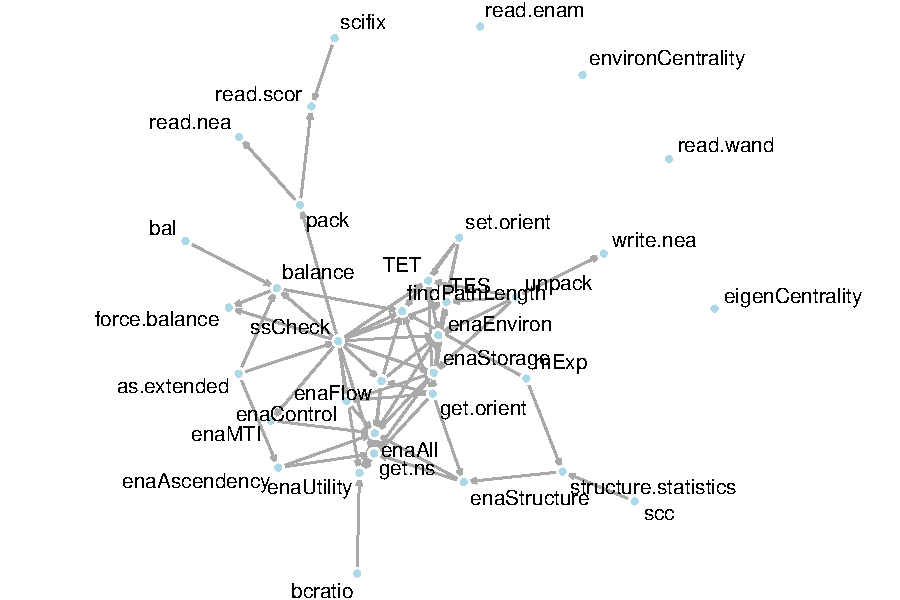
\includegraphics[]{enaR-vignette-003}
\caption{A plot of the \textit{enaR} function relationships. Edges
  point \textit{from} a function that provides information \textit{to}
  the function that receives that information.} \label{fig:fig}
\end{figure}

% % use
% The analysis has been used in a variety of ways, including to show the
% relative importance of indirect effects in ecosystems \citep{patten83,
%   higashi89, salas11_did} and their capacity to effectively transform
% the relations among organisms \citep{ulanowicz90, patten91, fath98,
%   bondavalli99}.  From these applications a new theoretical
% understanding of ecosystems has emerged \citep{higashi91, belgrano05,
%   jorgensen07_newecology}.  Recently, scientists have been applying
% these methods to understand trophic dynamics in the Sylt-R{\o}m{\o}
% Bight \citep{baird04_sylt,baird08_sylt}, biogeochemical cycling in
% estuaries \cite{christian03, hines12}, and urban sustainability
% \citep{zhang10, chen12}.

\section{Data Input: General}
In this section we describe the data necessary for the Ecological
Network Analysis and show how to build the central network data object
in \R\ that contains the model data for subsequent analysis.  To
start, we assume you have installed the enaR package, and then loaded
the library as follows:

%%%%% Getting Set Up %%%%%%%%%%%
\setkeys{Gin}{width=0.55\linewidth}

% Show loading the library and listing the functions in the package
\begin{Schunk}
\begin{Sinput}
> library(enaR)
\end{Sinput}
\end{Schunk}
%%%%%%%%%%%%%%%%%%%%%%%%%%%%%%%%%

\subsection{Model Data} \label{sec:data}
ENA is applied to a network model of energy--matter exchanges among
system components.  The system is modeled as a set of $n$ compartments
or nodes that represent species, species-complexes (i.e., trophic
guilds or functional groups), or non-living components of the system
in which energy--matter is stored.  Nodes are connected by $L$
observed fluxes, termed directed edges or links.  This analysis
requires an estimate of the energy--matter flowing from node $i$ to
$j$ over a given period, $\mathbf{F}_{n\times n}=[f_{ij}]$,
$i,j=1,2,\ldots,n$.  These fluxes can be generated by any process such
as feeding (like a food web), excretion, and death.  As ecosystems are
thermodynamically open, there must also be energy--matter inputs into
the system $\mathbf{z}_{1 \times n}=[z_i]$, and output losses from the
system $\mathbf{y}_{1 \times n}=[y_i]$.  While the Patten School treats
all outputs the same, the Ulanowicz School typically partitions
outputs into respiration $\mathbf{r}_{1\times n}=[r_i]$ and export
$\mathbf{e}_{1\times n}=[e_i]$ to account for differences in energetic
quality. Note that $y_i = r_i + e_i, \forall i$.  Some analyses
also require the amount of energy--matter stored in each node (e.g.,
biomass), $\mathbf{X}_{1\times n}=[x_i]$.  The final required
information is a categorization of each node as living or not, which
is essential for algorithms from the Ulanowicz School.  For
our implementation, we have created a logical vector $\mathbf{Living}_{1 \times
  n}$ that indicates whether the $i^{th}$ node is living (TRUE)
or not (FALSE).  Together, the model data $\mathcal{M}$ can be
summarized as $\mathcal{M} =
\{\mathbf{F}, \mathbf{z}, \mathbf{e}, \mathbf{r}, \mathbf{X}, \mathbf{Living}\}$.


% Orientation
The ENA methodology is an application and extension of economic
Input--Output Analysis \citep{leontief1936,leontief66} that was first
introduced into ecology by \citet{hannon73}.  Two major schools have
developed in ENA.  The first is based on Dr.\ Robert E.\ Ulanowicz's
work with a strong focus on trophic dynamics and a use of information
theory \citep{ulanowicz86, ulanowicz97, ulanowicz04}.  The second
school has an environment focus and is built on the environ concept
introduced by Dr.\ Bernard C.\ Patten \citep{patten76, patten78,
  fath99_review}.  Patten's approach has been collectively referred to
separately as \emph{Network Environ Analysis}. At the core the two
approaches are very similar; however, they make some different
starting assumptions and follow independent yet braided development
tracks. One example difference that has historically inhibited
collaboration and applications is that the two schools orient their
analytical matrices in different ways.  The Ulanowicz school orients
their matrices as flows from rows-to-columns, which is the most common
orientation in the broader field of network science
\citep[e.g.,][]{brandes05}.  In contrast, the Patten School has
historically oriented their matricies from column-to-row.  Recent
research has started to bring the work of the two schools back
together \citep[e.g.,][]{scharler09comparing}; we hope this software
contributes to this.  

Notice the row-to-column orientation of $\mathbf{F}$.  This is
consistent with the Ulanowicz School of network analysis, as well as
the orientation commonly used in Social Network Analysis and used in
the \textit{statnet} packages.  However, this is the opposite
orientation typically used in the Patten School of analysis that
conceptually builds from a system of differential equations and thus
uses the column-to-row orientation common in this area of
mathematics. Even though the difference is only a matrix transpose,
this single difference may be the source of much confusion in the
literature and frustration on the part of users.  We have selected to
use row-to-column orientation for our primary data structure, as it is
the dominant form across network analytics as evidenced by it use in
the \textit{statnet} packages. The package algorithms also return the
results in the row-to-column orientation by default; however, we have
built in functionality with the functions \texttt{get.orient} and
\texttt{set.orient}  that allows users
to return output in the Patten School row-to-column orientation
(see Section~\ref{sec:orient} for details).

% % Assumptions
% To validly apply flow analysis, the network model must meet two
% analytical assumptions.  First, the model must trace a single,
% thermodynamically conserved currency such as energy, carbon, or
% nitrogen.  Second, the model must be at steady-state for many of the
% analyses.  This means that the sum of the energy--matter flowing into
% a node equals that exiting the node such that its storage or biomass
% is not changing.  \citet{fath07_netconstruction} offer further
% suggestions for better ecosystem network model construction.

% Network Data Object
\subsection{Network Data Class}

The \textit{enaR} package stores the model data in the \textbf{network}
class defined in the \textit{network} package \citep[see][for
details]{butts08_network}. Again, the primary network object
components are:

\begin{itemize}
\item F = flow matrix oriented row-to-column
\item z = inputs
\item r = respiration
\item e = exports
\item y = respiration+exports
\item X = biomass or storage values
\item Living = logical vector indicating if the node is living
  (TRUE) or non-living (FALSE)
\end{itemize}

\subsection{Building a Network Object}
Users can assemble the necessary data elements described in
Section~\ref{sec:data} and then use the \texttt{pack} function to create the
network data object.  Here is an example of doing this with
hypothetical data.

%% PACK A MODEL
\begin{Schunk}
\begin{Sinput}
> # generate the flow matrix
> flow.mat <- array(abs(rnorm(100,4,2))*sample(c(0,1),100,replace=TRUE),
+                    dim=c(4,4))
> # name the nodes
> rownames(flow.mat) <- colnames(flow.mat) <- paste('node',(1:nrow(flow.mat)),sep='')
> # generate the inputs
> inputs <- runif(nrow(flow.mat),0,4)
> # generate the exports
> exports <- inputs
> # pack
> fake.model <- pack(flow=flow.mat,
+                     input=inputs,
+                     export=exports,
+                     living=TRUE)
\end{Sinput}
\begin{Soutput}
[1] "respiration" "storage"    
\end{Soutput}
\begin{Sinput}
> # model
> fake.model
\end{Sinput}
\begin{Soutput}
 Network attributes:
  vertices = 4 
  directed = TRUE 
  hyper = FALSE 
  loops = TRUE 
  multiple = FALSE 
  bipartite = FALSE 
  balanced = FALSE 
  total edges= 10 
    missing edges= 0 
    non-missing edges= 10 

 Vertex attribute names: 
    export input living output respiration storage vertex.names 

 Edge attribute names: 
    flow 
\end{Soutput}
\end{Schunk}

Unfortunately, the attributes() function does not clearly identify the
network data objects we are using.

\begin{Schunk}
\begin{Sinput}
> attributes(fake.model)
\end{Sinput}
\begin{Soutput}
$names
[1] "mel" "gal" "val" "iel" "oel"

$class
[1] "network"
\end{Soutput}
\begin{Sinput}
> 
\end{Sinput}
\end{Schunk}

However, individual components can be extracted from the data object
using the form specified in the \textit{network} package.  For
example, we can pull out node of vertex attributes as follows:

\begin{Schunk}
\begin{Sinput}
> fake.model%v%'output'
\end{Sinput}
\begin{Soutput}
[1] NA NA NA NA
\end{Soutput}
\begin{Sinput}
> fake.model%v%'input'
\end{Sinput}
\begin{Soutput}
[1] 3.2162867 3.7139823 2.6417828 0.2950702
\end{Soutput}
\begin{Sinput}
> fake.model%v%'living'
\end{Sinput}
\begin{Soutput}
[1] TRUE TRUE TRUE TRUE
\end{Soutput}
\end{Schunk}

For convenience, we have defined the flow matrix as a network based characteristic and it can be extracted as:

\begin{Schunk}
\begin{Sinput}
> fake.model%n%'flow'
\end{Sinput}
\begin{Soutput}
NULL
\end{Soutput}
\end{Schunk}

There are times that it is useful to extract all of the ecosystem
model data elements from the network data object.  This can be
accomplished using the \texttt{unpack} function. The \texttt{unpack}
output is as follows:

\begin{Schunk}
\begin{Sinput}
> unpack(fake.model)
\end{Sinput}
\begin{Soutput}
$F
         node1    node2     node3    node4
node1 0.000000 4.374742 0.2145385 0.000000
node2 7.124684 7.090482 0.0000000 1.933229
node3 0.000000 3.746494 3.9480187 4.476634
node4 0.000000 7.570623 6.5938201 0.000000

$z
[1] 3.2162867 3.7139823 2.6417828 0.2950702

$r
[1] 0 0 0 0

$e
[1] 3.2162867 3.7139823 2.6417828 0.2950702

$y
[1] NA NA NA NA

$X
[1] NA NA NA NA

$Living
[1] TRUE TRUE TRUE TRUE
\end{Soutput}
\end{Schunk}

Note that we did not specify the storage values. In these instances
\texttt{pack} produces \texttt{NA} values. Although the package is
designed to help users navigate missing data issues be sure to check that you
are providing the appropriate input for a given function. For more
information, see the help file for the function in question.

%%%%%%%%%%%%%%%%%%%%%
\subsection{Balancing for Steady-State}

Many of the ENA functions assume that the network model is at
steady-state (node inputs equal node outputs).  Thus, this package has
functions for (1) checking to see if the assumption is met and (2)
automatically balancing the model so that input equal outputs.

To determine if the model is balanced and then balance it if necessary:
\begin{Schunk}
\begin{Sinput}
> ## --- Check to see if the model is balanced ---#
> ssCheck(fake.model)
\end{Sinput}
\begin{Soutput}
[1] FALSE
\end{Soutput}
\begin{Sinput}
> ## --- To BALANCE a model if needed --- #
> fake.model <- balance(fake.model,method="AVG2")
\end{Sinput}
\begin{Soutput}
[1] AVG2
\end{Soutput}
\begin{Sinput}
> ## --- To FORCE BALANCE a model if needed --- #
> fake.model <- force.balance(fake.model)
\end{Sinput}
\end{Schunk}

The automated balancing routines are based on those presented in
\citet{allesina03}.  These authors compare alternative balancing
algorithms and further discuss the implications of using automated
procedures.  Caution is warranted when using these techniques, as they
indiscriminately alter the model flow rates.

%%%%%%%
\section{Data Input: Reading Common Data File Formats}
Several software packages exist in the literature for running ENA.  For
convenience, we have written functions to read in a few of the more
common data formats used by these software.

\subsection*{SCOR}
The \texttt{read.scor} function reads in data stored in the SCOR
format specified by \citet{ulanowicz91} that is the input to the
NETWRK4 programs.  This function can be run as follows.

\begin{Schunk}
\begin{Sinput}
> scor.model <- readLines('http://people.uncw.edu/borretts/data/oyster.dat')